\section{Свёрточные нейронные сети}


Свёрточные нейронные сети (convolutional neural network, CNN)- незаменимый инструмент для решения подавляющего большинства задач компьютерного зрения. 
На сегодняшний день существует множество различных архитектур, нацеленных на решения той или иной задачи. 
Очень часто свёрточные сети применяют как бекбон - сеть, которая предобучена извлекать признаки из изображения. К получившейся 
на выходе из такой сети карты признаков можно применять дополнительные преобразования для решения конкретной задачи. 

В рассмотренных нами подходах к решению задачи выявления заметных объектов на изображении свёрточные нейронные сети 
применяются и как самостоятельная модель(?), и в качестве бекбона. Однако, основные составные части свёрточной сети 
остаются практически неизменными. В этой главе будут описаны основные операции, характерные для архитектуры свёрточной нейронный сети,
а также рассмотрены архитектуры ResNet-50\cite{ResNet} и Efficient-Net b0 \cite{Efficientnet}, которые будут использованы в качестве 
бекбонов.

//TODO: два предложение чё такое карта признаков

Основные операции в свёрточнах нейронных сетях - это идущие последовательно свёртка, активация и пулинг. Блоки из свёртки и операции
обычно повторяются несколько раз перед применением пулинга \cite{ResNet}. Рассмотрим эти операции подробнее.
// TODO: слой или операция свёртки и остальные? 

\subsection{Операция свёртки}

Свёрточный слой - основной строительный блок свёрточной нейронной сети. Каждый слой свёртки содержит несколько ядер установленного размера,
обычно $3 \time 3$ или $5 \time 5$, каждое из которых применяется ко входной карте активации и с некотором шагом проходит по всей карте,
перемножая параметры ядра с параметрами входное карты вдоль всех каналов, а затем складывая их друг с другом и записывая в новую карту признаков.

// TODO: картинка!


// TODO побольше про dilaion rate: https://towardsdatascience.com/types-of-convolutions-in-deep-learning-717013397f4d

Обычно у свёртки рецептивное поле, то есть группа чисел в карте признаков, попадающая под действие свёртки,
соответствует форме и размеру ядра, например квадрату $3 \time 3$. Однако, существует более общий вид,
называемый расширенной свёрткой(Dilated Convolutions)\cite{Dilated}. У таких свёрток рецептивное поле контролируется параметром скорости
расширения (dilation rate). Так, для стандартной свёртки он равен 1. Если параметр равен 2, то рецептивное поле увеличивается
до размера $5 \time 5$, как показано на изображении \ref{fig:dilated}


\begin{figure}[h]
    \centering
    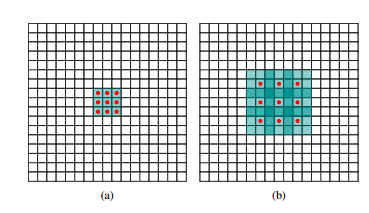
\includegraphics[width=1\textwidth]{dilated}
    \caption{Пример расшеренной свёртки. (a) параметр dilation rate равен 1, что соответствует обычной свёртке. (b) параметр dilation rate равен 2}
    \label{fig:dilated}
\end{figure}

\subsection{Пулинг}

Операция пулинга(Pooling), или операция субдискретизации, представляет собой операцию уменьшения размерности входящей карты признаков 
путём применения некоторой стратегии. Самой распространённой стратегией является стратегия максимально пулинга(Max Pooling),
при которой из группы соседних чисел, например внутри квадрата $2 \times 2$, выбирается максимальное и записывается в новую
карту признаков 

//TODO картинку!

Операция пулинга может быть записана следующим образом:

\begin{equation}
    f_{x,y}(S) = \max_{a,b=0}^{s}S_{sX+a, sY+b}
\end{equation}

где $S$ - карта активации, $s$ - размер окна.

\subsection{Функция активации ReLU}

Обычно, после применения свёртки, следующим шагом идёт применение функции активации для добавления нелинейности. Таким образом,
несколько последовательных свёрток, являясь линейными операциями, не будут эквивалентны одной свёртке, а будут описывать действительно 
разные признаки объекта. Одной из самых популярных функций активаций стала функция ReLU(Rectified Linear Unit), которая определяется
как.

\begin{equation}
    f(x) = max(0,x)
\end{equation}

//TODO: картиночка с функцией


\subsection{Про батч норму ещё!}
// TODO